\chapter{Experimental}

This chapter describes the apparatus at Colorado State University which has been used for all described studies of Ba/Ba\textsuperscript{+} fluorescence in SXe after deposition in vacuum.  Our main barium source, a Ba\textsuperscript{+} ion beam, is first described, as well as a purely Ba neutral source.  The co-deposit of Ba/Ba\textsuperscript{+} with Xe gas onto a cold sapphire window, subsequent laser excitation, and finally the collection optics for the fluorescence are described.

\section{Ion Beam}

The full ion beam is shown in Fig. \ref{fig:ionbeam}.  This is a clean source of Ba\textsuperscript{+} which can do a very wide range of deposit sizes, from billions of ions in a focused laser region all the way down to the single-ion level {\color{gray}, and even deposits sparse enough to scan a laser over spatially separated ions (may only want to say that if we have those scans)}.

\begin{figure} %[H]
        \centering
                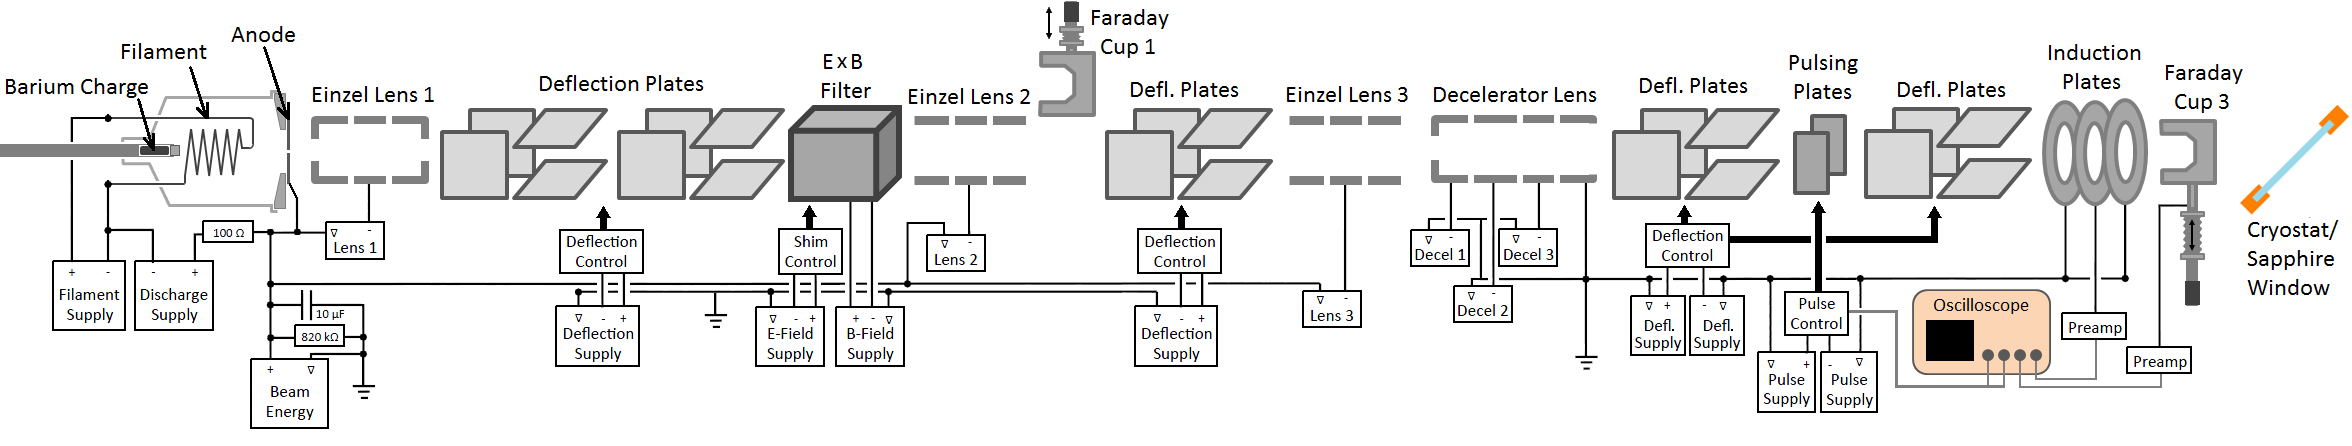
\includegraphics[angle=90,width=.25\textwidth]{figures/ionBeam.png}
                \caption{Ba\textsuperscript{+} ion beam.}
\label{fig:ionbeam}
\end{figure}

\subsection{Ion Source}

Ba\textsuperscript{+} ions are produced in a Colutron ion gun system \cite{Colutron}.  The source is shown in Fig. \ref{fig:ionsource}.  A solid barium charge is placed into the hollowed end of a stainless steel rod, which is then inserted into the discharge chamber, near the hot filament.  The barium vaporizes, and escapes the hollowed rod around a loosely threaded set screw.  The source is designed to produce a discharge between the anode plate and the filament cathode, through an argon buffer gas leaked into the source chamber.  This controlled discharge would then also ionize atoms from the solid charge to produce the desired ion beam, and Ar ions would be filtered out.  However, to avoid contamination of the SXe matrix with residual Ar gas, the buffer gas is not used in this work.  We are still able to maintain a discharge between the filament and anode circuits.  The longevity of ion current from a single charge (at least several 10s of hours) suggests that Ba is coating the inner walls of the chamber and is depleted slowly.  This is supported by the observation of white oxidation of the inner source parts after a few minutes of exposure to air when opening the system.  The discharge produces a plasma, containing barium ions, which escapes the chamber through a small hole in the anode, where it enters the acceleration region.  The acceleration potential is 2~kV, between the ion source anode and an aperture, which is the first element of Einzel lens 1.  This lens approximately collimates the ion beam for passage through the E$\times$B velocity filter.

\begin{figure} %[H]
        \centering
                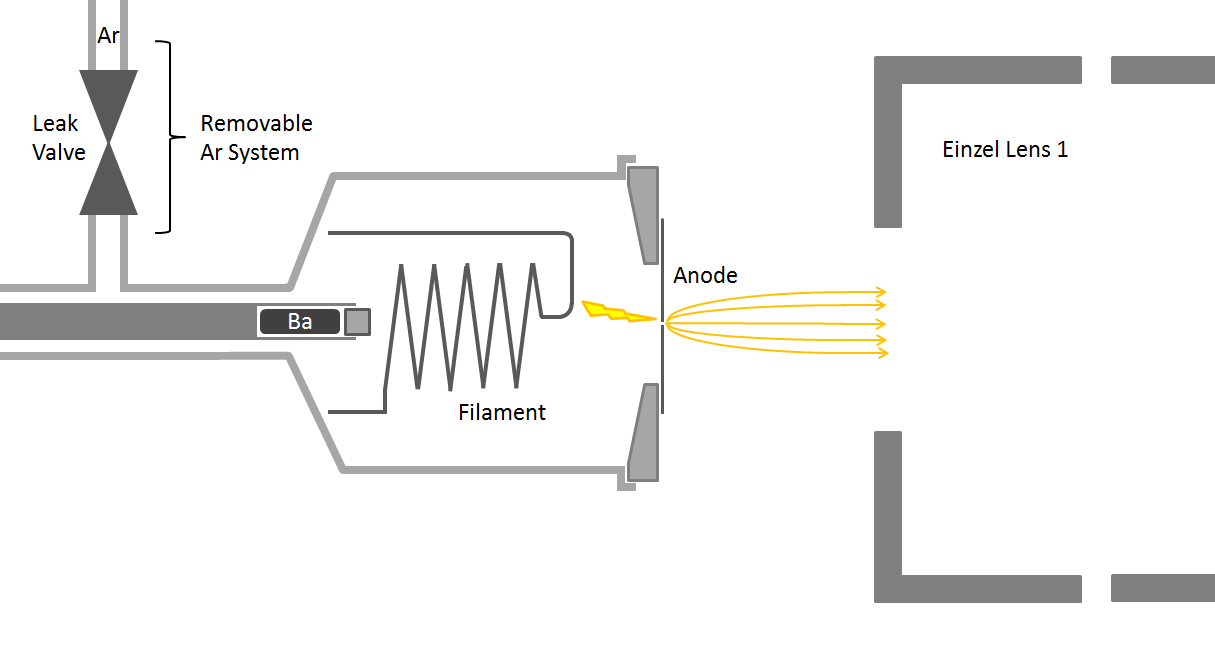
\includegraphics[width=.95\textwidth]{figures/ionSource.png}
                \caption{Ba\textsuperscript{+}/Ar\textsuperscript{+} ion source.}
\label{fig:ionsource}
\end{figure}

\subsection{E$\times$B Velocity Filter}

The E$\times$B velocity filter selects Ba\textsuperscript{+} by creating perpendicular electric and magnetic fields, which produce opposing forces on charged particles moving straight through the filter.  The opposing forces will be equal for ions with velocity $v = \frac{E}{B}$.  Since ion velocity is determined by mass ($m$), charge ($q$) and beam potential ($V$), the filter selects ions satisfying Eq. \ref{eqn:massfilt}:

\begin{equation}
\frac{m}{q} = \frac{2 V B^{2}}{E^{2}}
\label{eqn:massfilt}
\end{equation}

\noindent
where $B$ and $E$ are the magnetic and electric fields, respectively.  Those fields are chosen such that the forces are equal for Ba\textsuperscript{+}.  Other ions will be deflected.  

The E$\times$B filter is shown in Fig. \ref{fig:exb}.  Electromagnets provide the vertical magnetic field.  Electrode plates and field-shaping guard rings provide the horizontal electric field.  The guard rings prevent a lensing and astigmatism effect from fringe fields of the plates \cite{Colutron}.

\begin{figure}[h]
        \centering
                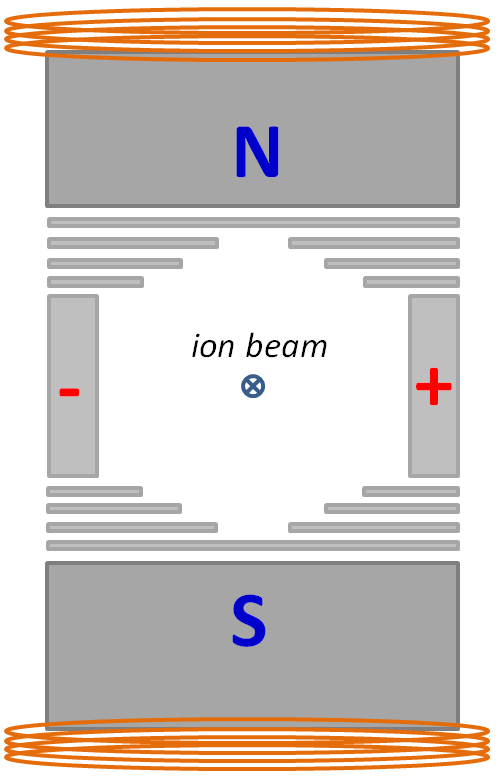
\includegraphics[width=.7\textwidth]{figures/ExB.png}
                \caption{Colutron E$\times$B ion velocity filter.}
\label{fig:exb}
\end{figure}

\emph{\color{gray}If we need mass scans, we probably need to do new ones with a constant magnetic field, and Ar\textsuperscript{+} and Ba\textsuperscript{+} in same day.  Past scans were all over the place, partly because we were changing beam settings, but new peaks are not very consistent either.}
%To determine the mass components of the beam, the electric field can be scanned.  Mass scans of the Ba\textsuperscript{+} beam is shown in Fig. [ref mass scan fig], as well as of an Ar\textsuperscript{+} beam.  The known mass of Ar aids in calibrating the magnetic field, which differs from the calculation given by Colutron, likely due to hysteresis in the magnet.  \emph{\color{gray}The Ba\textsuperscript{+} peak agrees with the Ba mas s... }

\subsection{Other Beam Components}

The first three sets of deflection plates can be used for beam diagnostics, and are set to 0~V during normal operation.  The deflection plates just before the pulsing plates, H1 and V1, are set to constant values of 50~V and 0~V, respectively, which have been selected such that the beam, in both pulsing and continuous modes, can be deposited at the sapphire window for reasonable settings on the final deflection plates, H2 and V2.  As described in \ref{subsec:ionDepCal}, different settings in H2/V2 are required for peak ion current in Faraday cup 3 vs. peak deposit at the window.

Einzel lens 2 focuses the beam the pass through the aperture in the first element of the decelerator lens.  Einzel lens 3 is not used in this setup.  The decelerator lens can be used to vary Ba\textsuperscript{+} deposit energy, but it in this work it acts as an Einzel lens with only the second element at voltage, and it focuses the beam at Faraday cup 3 (there is no Faraday cup 2 in this setup).  Faraday cup 3 measures the ion current during experiments, and is retracted when deposits are being made.  Its use in deposit calibration is described in \ref{subsec:ionDepCal}.  Faraday cup 1 is used for beam diagnostics, and is usually retracted on its bellows.  

\subsection{Ion Beam Pulsing}

When running in pulsing mode, the pulsing plates are first set to 200~V and -200~V to deflect the beam, and are pulsed to 0~V for 1~$\mu$s for each pulse.  The pulsing circuit is shown in Fig. \ref{fig:pulse_circuit}.  Square waves, triggered by LabVIEW at 500~Hz, enter the circuit at (a). The transformed pulse triggers the MOSFET switch, which closes the circuit for the period of the pulse.

\begin{figure} %[h]
        \centering
                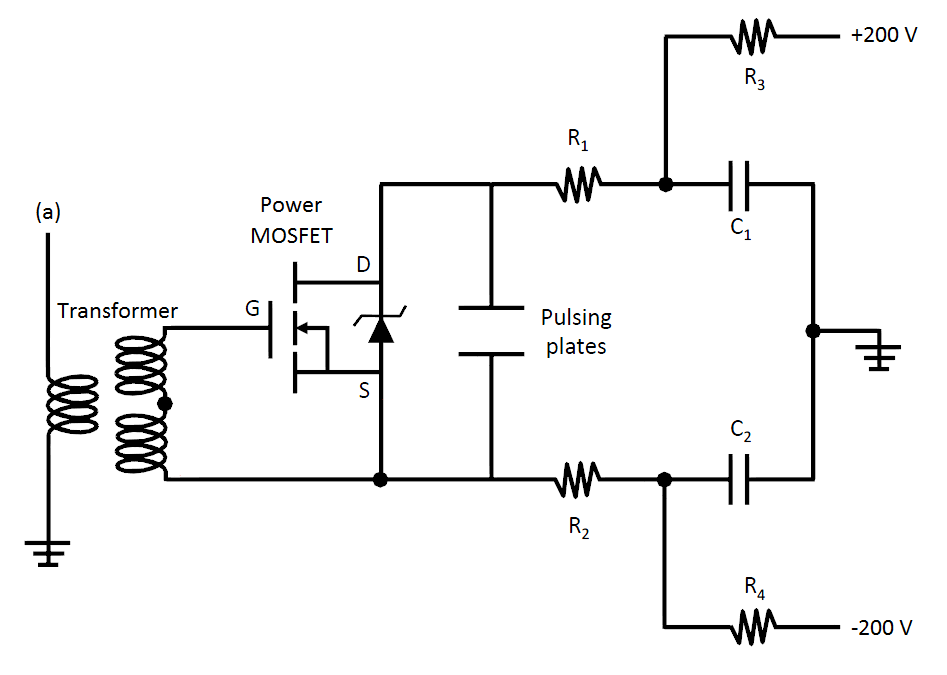
\includegraphics[width=.85\textwidth]{figures/pulsing_circuit.png}
                \caption{Pulsing circuit.  R$_{1}$ = R$_{2}$ = $470~\Omega$, R$_{3}$ = R$_{4}$ = 20~k$\Omega$, \newline C$_{1}$ = C$_{2}$ = 680~nF. \cite{Shon}}
\label{fig:pulse_circuit}
\end{figure}

The induction plates observe pulses during a deposit.  Pulses just prior to a deposit can be observed by cup 3 (as well as the induction plates) for a local measurement of ion current in the pulses.  eV Products pre-amplifiers convert the ion current to voltage signals which are read out with a digital oscilloscope.  An example of an oscilloscope readout of 16 averaged pulses is shown in Fig. \ref{fig:pulse_raw_shaped}(left).  The pre-amp circuit is solved to retrieve the original current, given by Eqn. \ref{eqn:preamp}:

\begin{equation}
I = \frac{-(V_{out} + R_{1} C \frac{dV_{out}}{dt})}{R_{1} M}.
\label{eqn:preamp}
\end{equation}

\noindent
$R_{1} C$ and $R_{1} M$ are determined for each pre-amp.  The time constant $R_{1} C$ is determined by fitting an exponential to the decay of a signal, and $R_{1} M$ is a constant which is then determined by fitting this shaped signal to a known input square pulse.  Final shaped currents for signals from the induction plates and cup 3 are shown in Fig. \ref{fig:pulse_raw_shaped}(right).

\begin{figure} %[H]
        %\centering
        %\begin{subfigure}
                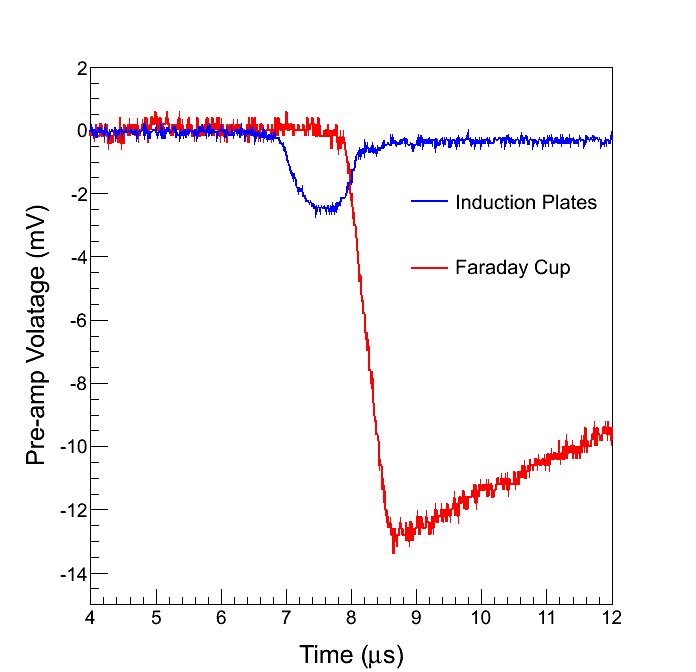
\includegraphics[width=.49\textwidth]{figures/pulse_ind_cup3_raw.png}
                %\caption{barf}
%        %\end{subfigure}
        %\begin{subfigure}
                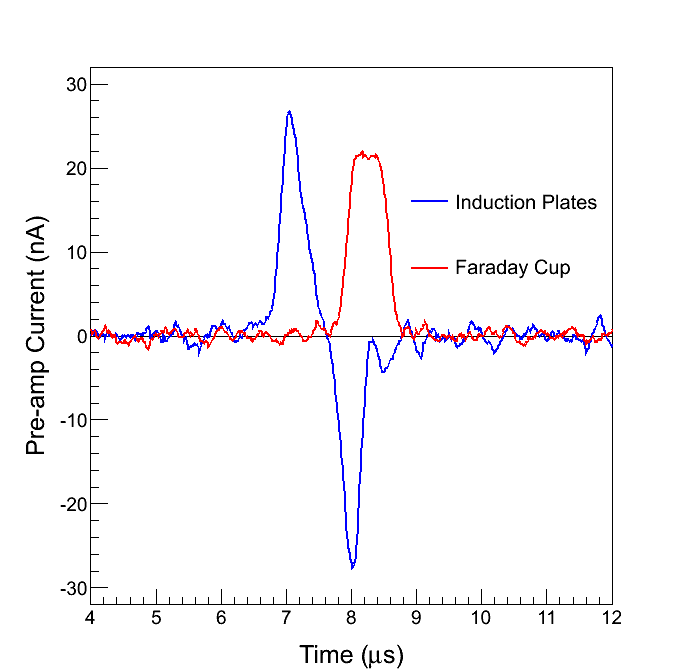
\includegraphics[width=.49\textwidth]{figures/pulse_ind_cup3_shaped.png}
                \caption{Raw (left) and shaped (right) pulse signals from induction plates and cup 3.  The raw induction signal appears small because it is a less sensitive pre-amp (accounted for in shaping).}
        %\end{subfigure}
        \label{fig:pulse_raw_shaped}
\end{figure}

Pulsing data also provides confirmation that the beam is composed of Ba\textsuperscript{+}.  The time between the center of the pulsing plate voltage overlap and the center of the pulse measured by the Faraday cup, along with a measurement of the distance traveled, provides a velocity measurement of the ions.  This distance was measured to be 31.5 $\pm$ 0.5~cm, and time-of-flight data, e.g. Fig. \ref{fig:pulses_ArBa}, give 39.8 $\pm$ 3.4~amu for Ar\textsuperscript{+} and 136.8 $\pm$ 6.3~amu for Ba\textsuperscript{+}, including an uncertainty on the time of flight of $\pm$ 0.1~$\mu s$.  This rules out any BaO\textsuperscript{+} contribution to the Ba\textsuperscript{+} ion beam.

\begin{figure}[h]
        \centering
                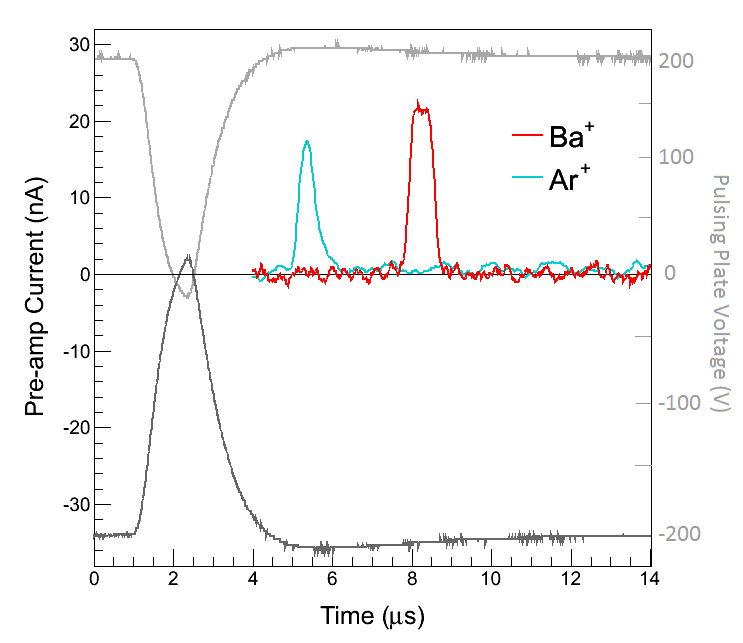
\includegraphics[width=.7\textwidth]{figures/pulses_BaAr.png}
                \caption{Arrival time of pulses at cup 3 vs. time of pulsing plate signal (black (+) and gray (-)) for Ar\textsuperscript{+} and Ba\textsuperscript{+}.}
\label{fig:pulses_ArBa}
\end{figure}

\subsection{Calibration of Ion Deposit}
\label{subsec:ionDepCal}

To calibrate the signal at cup 3 to an ion density at the sapphire window, another Faraday cup (cup w) is attached to the cold finger in place of the sapphire window.  Firstly, the ratio in $\frac{fC}{pulse}$ between cup 3 and cup w is measured ($\equiv f$).  Then, knowing the radius of cup w lets one determine the ion density per pulse at the sapphire window:

\begin{equation}
\frac{ions}{pulse \times m^{2}} = \frac{C f}{A e}
\label{eqn:ion_density}
\end{equation}

\noindent
where $C$ is $\frac{fC}{pulse}$ at cup 3, $A$ is the area of cup w, and $e$ is the elementary charge.  The required settings of the final deflection plates H2 and V2 are also determined by cup w.  These typically differ from the peak values for cup 3 by about 70~V in H2 and 60~V in V2, corresponding to about 4~mm in x and y position at cup w.

\section{Ba Getter Source}

BaAl$_{4}$ getters are neutral Ba sources typically used to grab reactive gas molecules in purifiers and vacuum tubes.  \emph{\color{red}don't say we, and look up how they work ... is it a rxn even in the non-Ni-powder case (our wire)?}We can use a getter as a source of neutral Ba.  It is very helpful to have a completely different Ba source, especially a neutral-only source, in identifying observed fluorescence peaks.  This is discussed further in \ref{subsec:peakIdentify}.

The getter used briefly in this work is an endothermic ... getter wire ... {\color{gray}[describe it]} ... show diagram, maybe also of it in the system at same position as cup 3.

\section{Sample Deposition}

The Ba\textsuperscript{+}/Ba is co-deposited with ultra-pure Xe gas onto a cold sapphire window.  Sapphire has good thermal conductivity at low temperature and good optical transparency in the visible.  The window is held to a coldfinger and is tilted at 45$^{\circ}$ to allow access of the ion beam as well as the excitation laser and collection optics.  To begin a deposit, Xe gas is flowed toward the window via a leak valve.  Cup 3 is then retracted to clear the path for Ba\textsuperscript{+} ions, which land in the SXe matrix as it grows.  Cup 3 is then replaced, and the Xe leak stopped.

\begin{figure} %[h]
        \centering
                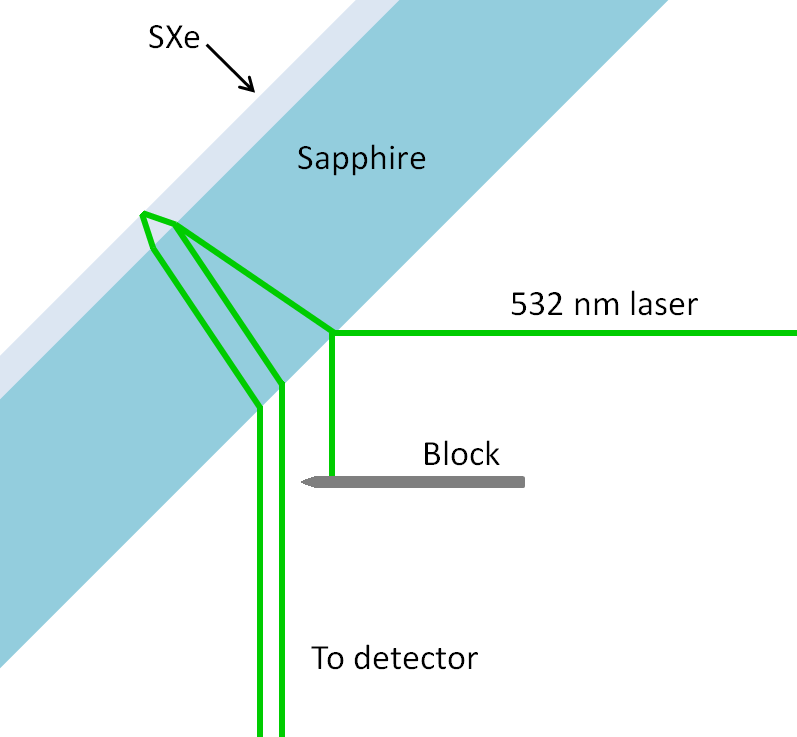
\includegraphics[width=.4\textwidth]{figures/fringe_setup.png}
                \caption{Setup for measuring SXe growth rate by interference fringes.}
\label{fig:fringe_setup}
\end{figure}

SXe matrix growth rate can be measured by interference fringes in a laser reflected against the front surface of the sapphire window, as shown in Fig. \ref{fig:fringe_setup}.  Fringes for SXe deposition at 52~K and 11~K are shown in Fig. \ref{fig:fringes_52K_vs_11K} for the leak rate used in this work.  The refractive index of SXe has a negligible dependence on temperature between 50~ and 30~K \cite{SXeIndex}, so these can be compared directly.  A somewhat lower rate is observed at 52~K, at 31~nm/s, vs. 37~nm/s at 11~K.  To evaporate a sample, the window is heated to around 100~K, and fringes also appear during this process as well.  The full set of fringes for a deposit at 52~K and its evaporation when heated is shown in Fig. \ref{fig:fringes_melt_withDep}, along with the window temperature.  This shows that the SXe evaporates between 73~K and 78~K.  Notice that the same number of fringes appear in the deposit and the evaporation.

\begin{figure} %[h]
        \centering
                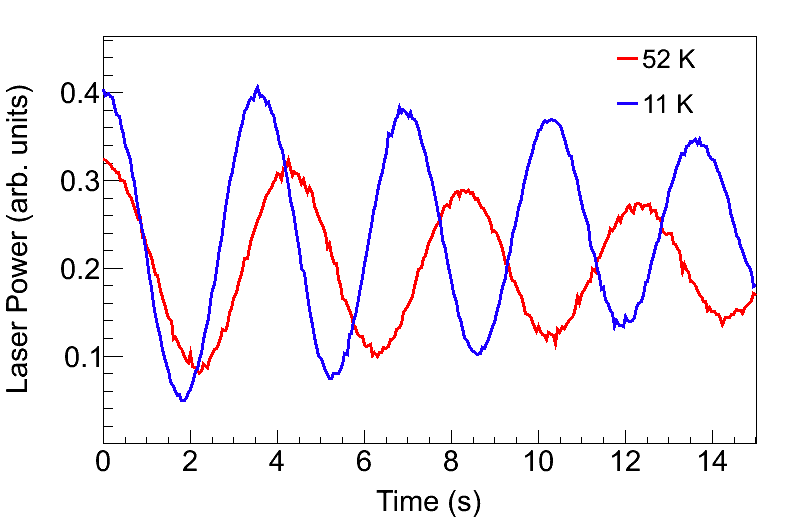
\includegraphics[width=.7\textwidth]{figures/fringes_52K_vs_11K.png}
                \caption{Interference fringes for the same Xe gas leak rate deposited on the sapphire window at 11~K and at 52~K.}
\label{fig:fringes_52K_vs_11K}
\end{figure}

\begin{figure} %[h]
        \centering
                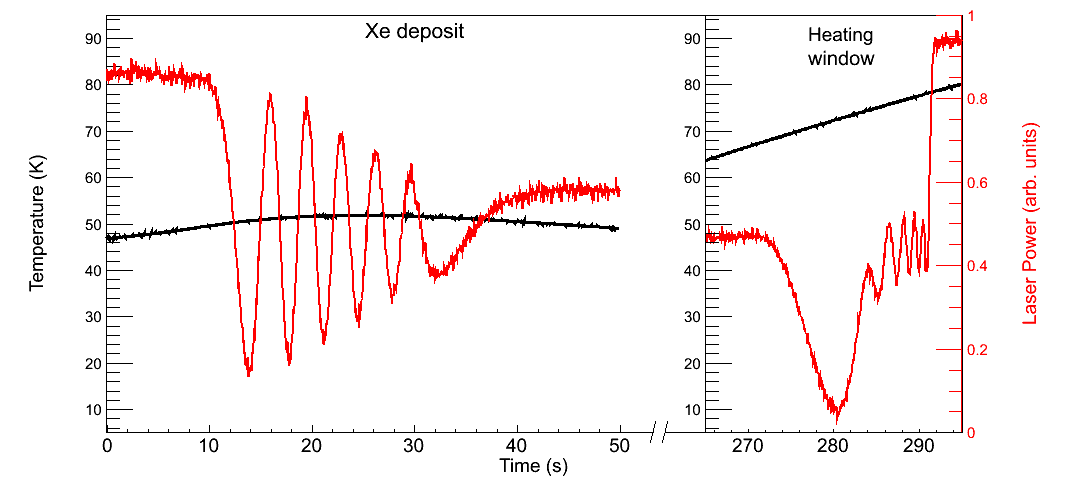
\includegraphics[width=.9\textwidth]{figures/fringes_dep_and_melt.png}
                \caption{Interference fringes of a deposit at 52~K and of its subsequent evaporation when heating the sapphire window.}
\label{fig:fringes_melt_withDep}
\end{figure}

\section{Laser Excitation}

Green/yellow light ... Coherent 599 dye laser ... R110 does ~542 - 566~nm, R6G does

[astigmatism in window, and data for that with compensator]

[also could put in the astigmatism check on the laser itself (consistent w/ zero) (pg. 24 of Chris's book)]

[waist measurements -- apply calibration uncertainty to the good motor-stage ones]

\section{Collection Optics}

talk about all that, including spectrometer